\chapter{提案手法}
\section{提案手法の概要}
本研究は, 技能伝承の現場において, 熟練技能者の持つ知識を継続的に抽出・共有できる持続可能な仕組みを確立することを目指す. これは, SECIモデルにおける「表出化」と「連結化」のプロセスに焦点を当て, 特に形式知化が可能な領域での知識抽出手法の確立を意味する.

「知識発現」\cite{Nishimura2017}をはじめとする従来の知識抽出手法では, 日常的な活動として知識抽出を継続的に行うことが困難であった. 本研究ではこの課題に対し, 技能の指導現場に着目し, LLMを活用した複合的なアプローチを提案する. 

具体的には, 以下の3つの要素を組み合わせることで, 日常的な知識抽出の仕組みを実現する:
\begin{enumerate}
    \item 知識の基盤 : 西村らの研究で提案されたプロセス知識の考え方を基礎とし, 知識工学の手法を用いて体系的に整理する
    \item 指導現場での対話収集 : 指導者と学習者の自然なやりとりから, まだ言語化されていない知識を抽出する
    \item LLMを用いた支援 : 収集した対話を分析し, 基盤となる知識の改良点を提案する
\end{enumerate}

これにより, 日常的な指導活動の中で知識を抽出しながら, LLMによる分析支援のもと, 熟練技能者が知識を整理・構造化することが可能となる. なおこれ以降, 本稿では技能伝承の文脈において熟練技能者を指導者と表記する. 以下, 提案手法の詳細について説明する.

\section{提案手法の仕組み}
本提案手法の全体像を図\ref{fig1}に示す. 先述の通り, 指導現場での日常的なインタラクションを通じて知識を抽出・構造化する.

まず, 指導対象となる技能についてのベースとなるプロセス知識を作成する. これは教科書や既存のマニュアルなどの形式知をもとに, 指導者の協力を得ながら構築する. このベースとなるプロセス知識は, 以降の知識抽出・構造化の土台となる. 

次に, 指導者の発言を自動的にロギングする. これには指導内容だけでなく, 学習者の理解度に応じた補足説明や, 予期せぬ質問への応答なども含まれる. 同様に, 学習者からの質問や感想といった応答も自動的に記録する. これらの対話ログは, 指導現場での暗黙的な知識のやり取りを捉える重要な情報源となる. 

収集された対話ログは, 既存のプロセス知識と併せてLLMによって解析される. LLMは対話の文脈を理解し, 現在のプロセス知識に不足している要素や, より詳細な説明が必要な箇所を特定する. そして, これらの分析結果に基づいて, プロセス知識の改良点を指導者に提案する. 

指導者はLLMからの提案を参考に, プロセス知識を改良することができる. ただし, この改良はLLMからの提案に限定されず, 指導者が日々の指導の中で気づいた点があれば, 随時プロセス知識を更新することも可能である. 

一方, 学習者もプロセス知識を参照することで, 指導内容への理解を深めることができる. これは単なる知識の参照に留まらず, 学習者からの新たな質問や気づきを生み出すきっかけともなり, さらなる知識の抽出・構造化のサイクルにつながっていく. 

このように, 提案手法は指導現場での自然なやりとりを起点として, LLMによる支援のもと, 継続的に知識を抽出・構造化していく仕組みを実現する. 

\begin{figure}[htbp]
    \centering
    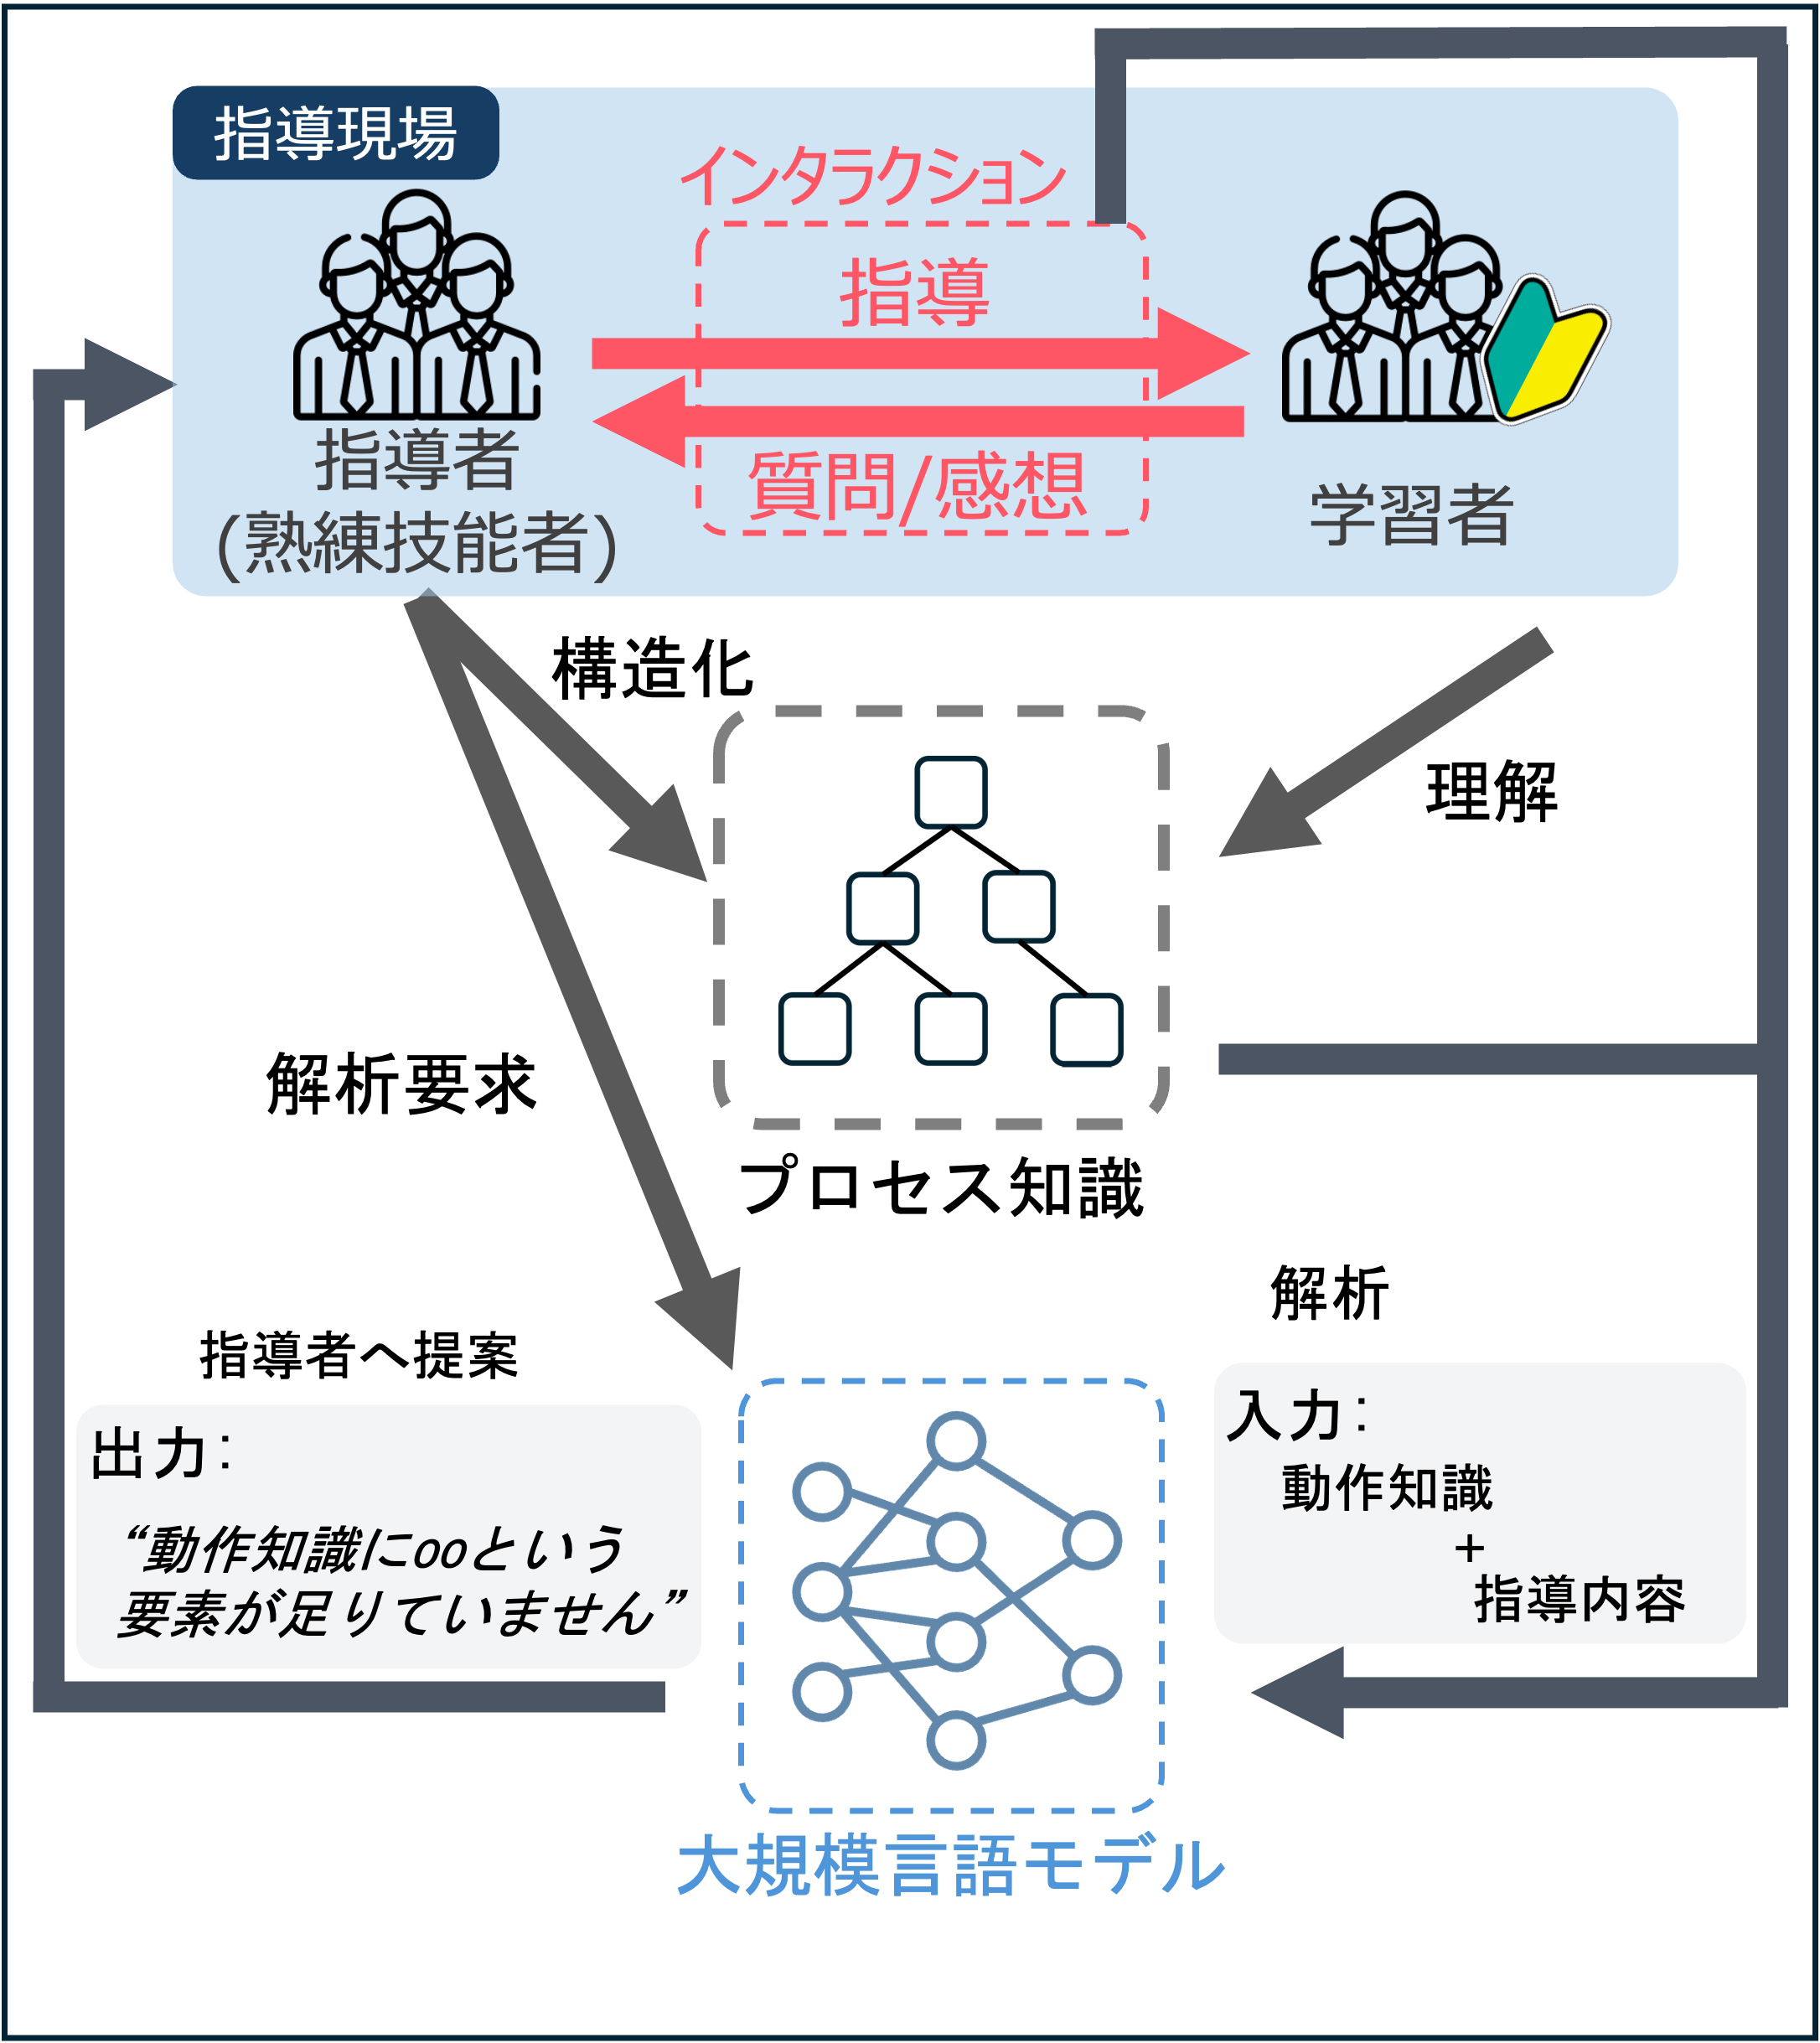
\includegraphics[width=0.9\linewidth]{./image/overview_2.png}
    \caption{提案手法の全体像}
    \label{fig1}
\end{figure}
